\section{Supplementary Results and Analysis}
\FloatBarrier

\subsection{Detailed Dataset Description}
\label{app:datasets}

The experiments use five MedMNIST v2 benchmarks~\cite{yang2023medmnist}. They were selected to cover microscopy, dermoscopy, CT, and ultrasound while varying the number of diagnostic classes and the prevalence profile. Table~\ref{tab:dataset-statistics} reports the exact split sizes used by the experiments; the descriptions below clarify the recognition problem represented by each benchmark.

\paragraph{Blood.} BloodMNIST is an eight-class microscopy benchmark for recognizing peripheral blood-cell morphology. Its classes include granulocytes, lymphocytes, and other cells with visually similar staining patterns. Fine-grained morphology makes it a useful stress test for whether a merged classifier preserves class-specific directions rather than concentrating its predictions on a small subset of cells.

\paragraph{Derma.} DermaMNIST contains seven dermoscopic skin-lesion categories. Its prevalence is strongly imbalanced and several categories share colour and texture patterns. This setting tests whether a merger distinguishes rare lesions without erasing the clinically meaningful prevalence of common lesions.

\paragraph{Organ-C and Organ-S.} OrganCMNIST and OrganSMNIST provide 11-way abdominal CT organ recognition in coronal and sagittal views, respectively. The two views share the same broad task but change the visible anatomy and image geometry, testing robustness across CT planes.

\paragraph{Ultrasound.} UltrasoundMNIST is an eight-class ultrasound-structure benchmark. Speckle noise, low contrast, and view-dependent boundaries make it particularly suitable for the prediction-collapse diagnostics and the per-class gap visualization in Fig.~\ref{fig:visual-chaosheng_predict}.

\begin{center}
\captionof{table}{BloodMNIST label space used in the experiments. The class IDs agree with the labels in the benchmark NPZ file.}
\label{tab:blood-labels}
\small
\renewcommand{\arraystretch}{1.12}
\begin{tabular}{clcl}
\noalign{\hrule height 1.25pt}
\rowcolor[HTML]{F2F2F2}
\textbf{ID} & \textbf{Class} & \textbf{ID} & \textbf{Class} \\
\hline \hline
0 & Basophil & 4 & Lymphocyte \\
\rowcolor{gray!10}
1 & Eosinophil & 5 & Monocyte \\
2 & Erythroblast & 6 & Neutrophil \\
\rowcolor{gray!10}
3 & Immature granulocyte & 7 & Platelet \\
\noalign{\hrule height 1.25pt}
\end{tabular}
\end{center}

\begin{figure*}[!t]
\centering
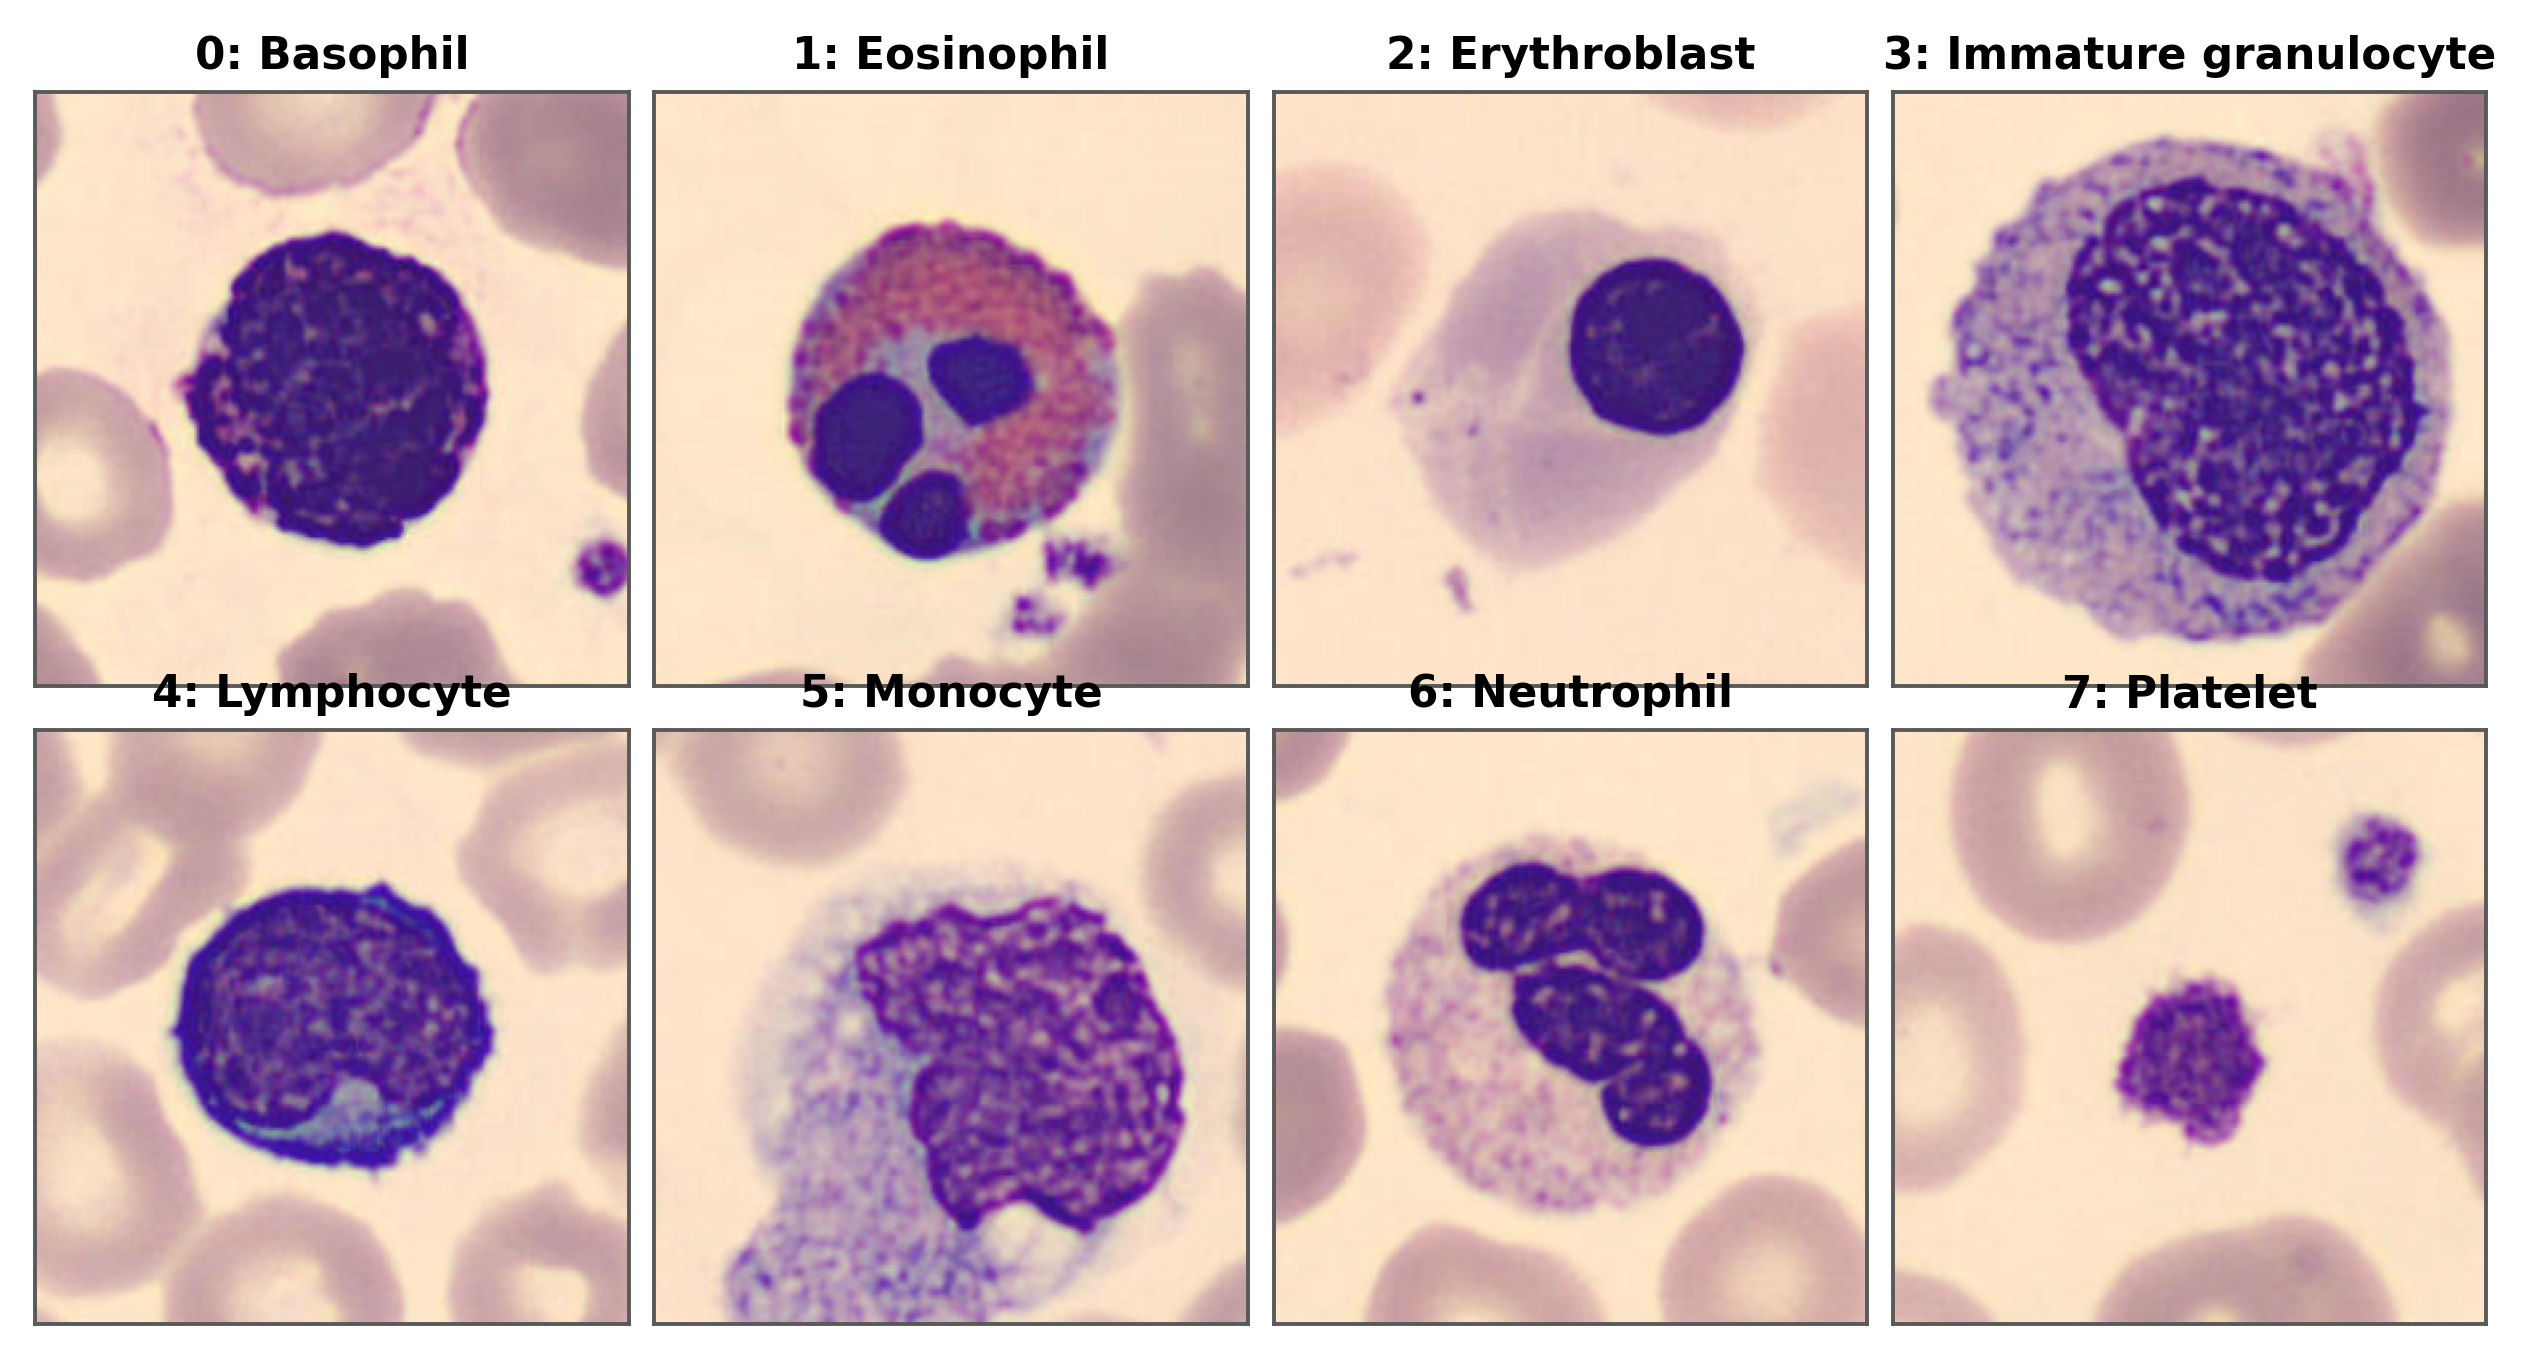
\includegraphics[width=0.93\textwidth]{figures/appendix_blood_classes.png}
\caption{Representative BloodMNIST training examples, one for every class in Table~\ref{tab:blood-labels}. Images are drawn directly from the labeled benchmark file used to construct the experimental partitions; they are shown only to document class appearance, not as training data for merging.}
\label{fig:blood-class-reference}
\end{figure*}

\subsection{Detailed Ablation Configurations and Interpretation}
\label{app:ablation-configurations}

All internal ablations use the same five datasets, four backbones, client counts, and Dirichlet settings as the main experiment. Thus, a change in Table~\ref{tab:diagnostic-internal-ablation} or Table~\ref{tab:prevalence-internal-ablation} isolates one design choice while holding the remaining LAMP-Merge pipeline fixed.

\subsubsection{Diagnostic Prototype Reconstruction}

For class \(c\), DPR aggregates reference-space prototypes as
\begin{equation}
p_c=\sum_{i=1}^{K}\alpha_{i,c}\mu_{i,c},\qquad
\alpha_{i,c}=\frac{e_{i,c}}{\sum_j e_{j,c}}.
\label{eq:appendix-dpr}
\end{equation}
\begin{equation}
e_{i,c}=(n_{i,c}+1)^\gamma\mathbf{1}[n_{i,c}>0].
\end{equation}
Here \(\mu_{i,c}\) is client \(i\)'s class-conditional reference-space mean and \(n_{i,c}\) is its support for that class. The substitutions below test whether the class semantics in \(\mu_{i,c}\) and the class-specific reliability in \(\alpha_{i,c}\) are both required.

\paragraph{Classifier-head aggregation (CHA).} CHA replaces the reference-space evidence by the local classifier-head direction, \(\mu_{i,c}\leftarrow h_{i,c}\). It tests whether client heads already provide a common, class-aligned representation. Its mean ACC is 25.63\%, a 36.58-point reduction from LAMP-Merge (62.21\%), showing that independently trained head directions are not a reliable substitute for shared-space class evidence.

\paragraph{Global-feature mean (GFM).} GFM removes class conditioning by using the same class-agnostic feature mean for every class, \(\mu_{i,c}\leftarrow g\). This tests whether generic client appearance alone can drive merging. Its 26.50\% mean ACC is 35.71 points below LAMP-Merge, indicating that class conditioning, not merely feature aggregation, is essential.

\paragraph{Support-only synthetic head (SSH).} SSH removes image-derived prototype information and sets \(p_c\leftarrow u_c\), where \(u_c\) is a fixed random unit vector. It preserves the classifier interface while eliminating diagnostic content. The 10.89\% mean ACC, 51.32 points below LAMP-Merge, verifies that performance does not arise from support counts or the cosine-head form alone.

\paragraph{Shuffled-label prototype (SLP).} SLP preserves prototype magnitudes but destroys their label correspondence, \(p_c\leftarrow p_{\sigma(c)}\), for a permutation \(\sigma\) of the diagnosis labels. Its 19.57\% mean ACC (a 42.64-point reduction) directly tests semantic alignment: useful class evidence must be assigned to the correct output class.

\paragraph{Uniform client weight (UCW).} UCW retains class prototypes but weights every client observing \(c\) equally:
\begin{equation}
\alpha_{i,c}\leftarrow\frac{\mathbf{1}[n_{i,c}>0]}{\sum_j\mathbf{1}[n_{j,c}>0]}.
\end{equation}
It tests whether observing a class is sufficient, independent of the amount of evidence. Its 58.33\% mean ACC is 3.88 points below LAMP-Merge, showing that support magnitude provides useful reliability information beyond class presence.

\paragraph{Binary support only (BSO).} BSO turns both prototype support and prevalence counts into presence indicators, \(n_{i,c},m_{i,c}\leftarrow\mathbf{1}[n_{i,c}>0]\). It tests whether fine-grained class frequency is necessary in both modules. The mean ACC falls to 55.18\% (7.03 points below LAMP-Merge), the largest loss among the weighting controls.

\paragraph{Global client-size weight (GCSW).} GCSW replaces class-specific reliability by total client size, \(e_{i,c}\leftarrow(N_i+1)^\gamma\mathbf{1}[n_{i,c}>0]\), where \(N_i=\sum_k n_{i,k}\). It tests whether a generally large client can stand in for strong evidence of a particular class. Its 59.39\% mean ACC, 2.82 points below LAMP-Merge, shows that local data volume should be assigned at the class level.

\paragraph{DPR summary.} The semantic controls cause large reductions (35.71--51.32 points), while the weighting controls cause smaller but consistent reductions (2.82--7.03 points). Together, these results support the two parts of Eq.~\ref{eq:appendix-dpr}: class-conditioned shared-space evidence provides the discriminative direction, and class-specific support determines how reliably each client contributes to that direction.

\subsubsection{Long-tail Prevalence Calibration}

LPC estimates an empirical prior and adds a centered, gated log-prior bias after DPR:
\begin{equation}
\pi_c=\frac{\sum_i m_{i,c}}{\sum_k\sum_i m_{i,k}},\qquad
b_c=\lambda\left(\log\pi_c-\frac{1}{C}\sum_k\log\pi_k\right).
\label{eq:appendix-lpc}
\end{equation}
\begin{equation}
\ell_c(x)=w_c^\top\phi_0(T(x))+\mathbf{1}[r>\tau]b_c.
\end{equation}
The three controls retain DPR and test the prior estimator or the activation gate in Eq.~\ref{eq:appendix-lpc}.

\paragraph{Uniform prevalence prior (UPP).} UPP suppresses prevalence information by setting \(\pi_c\leftarrow1/C\). It tests whether calibration should ignore the observed class distribution. Mean ACC is 58.91\%, 3.30 points below LAMP-Merge, demonstrating that the empirical prior is useful rather than a source of collapse.

\paragraph{Always-on calibration (AOC).} AOC removes the long-tail criterion and sets \(\mathbf{1}[r>\tau]\leftarrow1\). It tests whether the prior should be applied uniformly to every configuration. Its 61.90\% mean ACC is 0.31 points below LAMP-Merge. The small aggregate gap indicates that calibration is broadly useful, while the gated design avoids imposing a prior when a configuration is not sufficiently long-tailed.

\paragraph{Client-balanced prior (CBP).} CBP gives every client equal prior influence:
\begin{equation}
\pi_c\leftarrow\frac{1}{K}\sum_i\frac{m_{i,c}}{\sum_k m_{i,k}}.
\end{equation}
It tests whether each client should contribute equally regardless of sample volume. The 58.97\% mean ACC, 3.24 points below LAMP-Merge, favors the sample-count empirical prior over a client-balanced estimate.

\paragraph{LPC summary.} Every LPC control is below the 62.21\% LAMP-Merge mean. UPP and CBP show that both prevalence information and its sample-size weighting matter; AOC shows that the activation criterion is a targeted safeguard rather than the primary source of the gain. Hence LPC calibrates DPR's restored class directions instead of replacing them with a prior.

\subsection{Additional Analysis of DPR and LPC}

\subsubsection{Prototype estimation and class margins}

Let \(\mu_c^\star\) be the population class mean in the shared reference space. For client-level class estimates with bounded second moments, the mean-squared error of the aggregated prototype obeys
\begin{equation}
\mathrm{E}\|p_c-\mu_c^\star\|_2^2
\leq\sum_i\alpha_{i,c}^2\frac{\sigma_c^2}{n_{i,c}}+\mathrm{Bias}_c^2.
\label{eq:prototype-bound}
\end{equation}
The first term is a variance contribution: it decreases with support \(n_{i,c}\), but only clients that observed class \(c\) may contribute. The second term represents systematic mismatch between a local class estimate and the shared-space population mean. Equation~\ref{eq:prototype-bound} explains both support-related controls: UCW ignores unequal estimation variance, whereas GCSW confuses total client size with the support relevant to class \(c\).

For a reference feature \(z=\phi_0(T(x))\), consider two candidate classes \(c\) and \(d\). The population margin is
\begin{equation}
\Delta_{c,d}(x)=(\mu_c^\star)^\top z-(\mu_d^\star)^\top z.
\end{equation}
If
\begin{equation}
\|p_c-\mu_c^\star\|_2+\|p_d-\mu_d^\star\|_2
<\frac{\Delta_{c,d}(x)}{\|z\|_2},
\label{eq:margin-condition}
\end{equation}
then the reconstructed prototypes preserve the ordering between \(c\) and \(d\). Thus, class-specific aggregation is not intended to reproduce arbitrary local heads: it reduces prototype error sufficiently to retain discriminative class margins. The large losses for CHA, GFM, SSH, and SLP are consistent with breaking precisely this semantic margin mechanism.

\subsubsection{Bounded prevalence correction}

The centering in Eq.~\ref{eq:appendix-lpc} removes the uniform component of the log prior. Therefore only relative scores change, with
\begin{equation}
b_c-b_d=\lambda\log\frac{\pi_c}{\pi_d}.
\end{equation}
The gate \(\mathbf{1}[r>\tau]\) applies this relative correction only under sufficient prevalence imbalance, and the finite \(\lambda\) bounds its magnitude. DPR consequently supplies the class directions, while LPC adjusts the decision boundary only when the empirical class prevalence provides relevant evidence. This division also explains why a prevalence-only mechanism cannot solve the semantic controls in Table~\ref{tab:diagnostic-internal-ablation}.

\subsection{Metric Definitions}
\label{app:metric-geometry}

Let \(y_n\) and \(\hat{y}_n\) denote the true and predicted labels of sample \(n\), respectively. Let \(q_c=N^{-1}\sum_n\mathbf{1}[\hat{y}_n=c]\) be the predicted class distribution and \(p_c=N^{-1}\sum_n\mathbf{1}[y_n=c]\) the true distribution. The prediction-collapse diagnostics are
\begin{equation}
\rho=\max_c q_c,\qquad
C_{\mathrm{eff}}=\exp\left(-\sum_cq_c\log q_c\right).
\end{equation}
\begin{equation}
\mathrm{TV}(q,p)=\frac{1}{2}\sum_c|q_c-p_c|.
\end{equation}
The collapse ratio \(\rho\) measures the largest predicted-class share, \(C_{\mathrm{eff}}\) measures the effective number of classes used by the predictor, and TV measures distributional disagreement with the labels. Lower \(\rho\) and TV and higher \(C_{\mathrm{eff}}\) are preferred. The absolute per-class gaps in Fig.~\ref{fig:visual-chaosheng_predict} are \(|q_c-p_c|\) in percentage points and expose which classes contribute to TV.

\subsection{Hyperparameter-Sweep Reproducibility}

Every point in Fig.~\ref{fig:hparam-analysis} is a completed full-configuration experiment covering five datasets, four backbones, three client counts, and three Dirichlet settings (180 raw cells, or 60 client-average cells after averaging the three skew levels). The plotted curves retain measured points in ascending parameter order; no smoothing, interpolation, or best-run selection is applied. The LPC grid records \(\tau\in\{2.0,2.5,3.0\}\) and calibration strengths \(\lambda\in\{3.00,3.25,\ldots,5.25\}\), with \(\gamma=0.55\) and \(s=18.75\) fixed. DPR completion records are read from the full-configuration run directories and are plotted only after all 180 cells have succeeded. The selected operating point is \(\gamma=0.55\), \(s=18.75\), \(\tau=2.5\), and \(\lambda=4.25\), making its reported value traceable to the same completed grid as its neighboring points.
